\documentclass[12pt]{article}
\usepackage{fullpage,enumerate,amsmath,amssymb,graphicx, float}

\begin{document}
\begin{center}
{\Large CS224N Fall 2014 Programming Assignment 2}
\vspace{12pt}

SUNet ID: tzhang54, jiajihu

Name: Tong Zhang, Jiaji Hu
\vspace{12pt}
\end{center}

\section{Implementing a CKY Parser}
\subsection{Algorithm and Naive Implementation}

\subsection{Optimizations}

\subsection{Results}
\subsubsection{Run Time}
\begin{center}
\begin{tabular}{|c|c|c|c|}
\hline
Algorithm & Total Runtime (s) & Avg. Runtime (s) & Length 20 (s)\\\hline
Basic & 185.48 & 1.20 & 2.56 \\\hline

\end{tabular}
\end{center}
\begin{figure}[H]
\centering
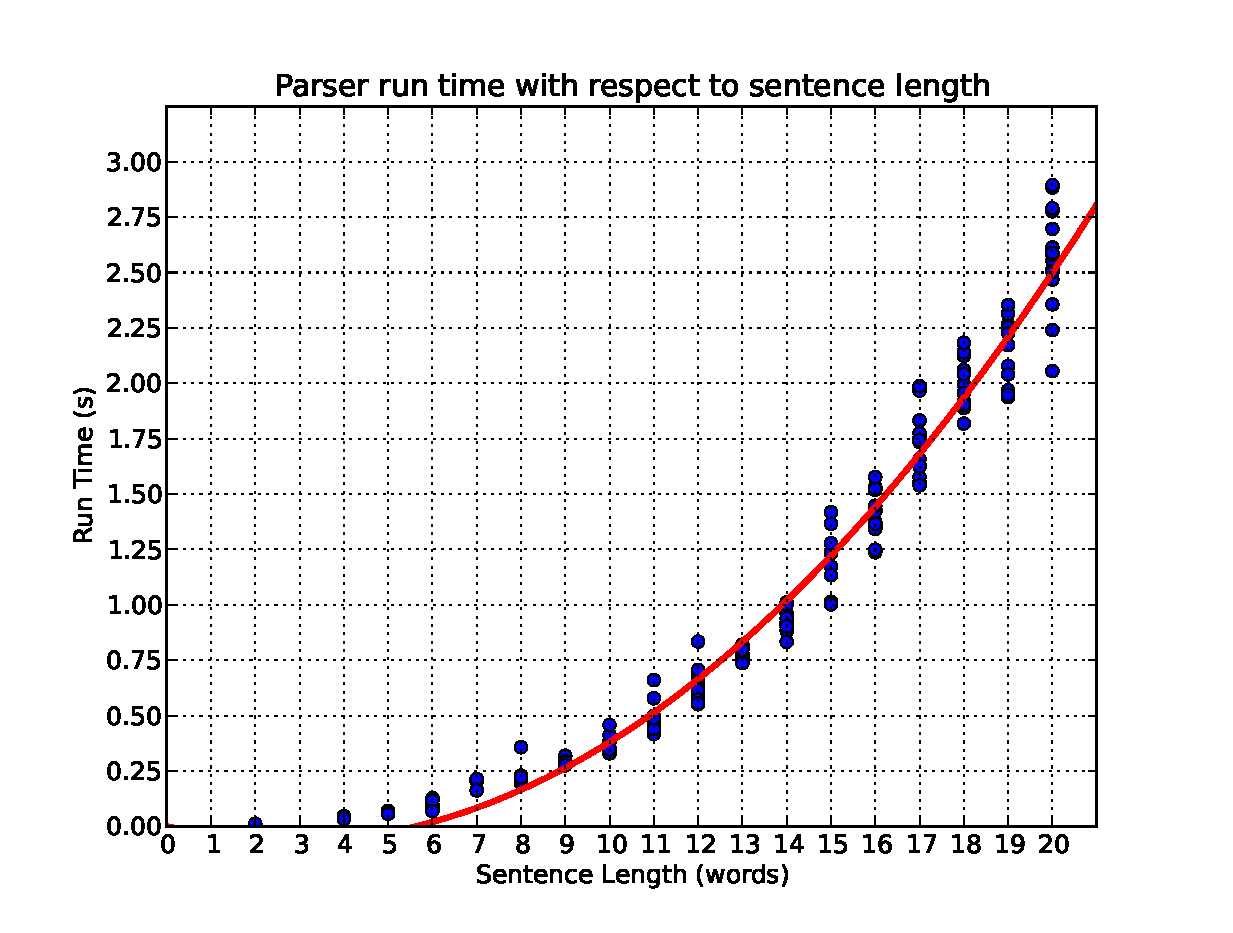
\includegraphics[width=0.6\linewidth]{./stats/runtime}
\end{figure}

\subsubsection{Parsing Score}
\begin{center}
\begin{tabular}{|c|c|c|c|c|}
\hline
Algorithm & Precision & Recall & $F_1$ & Exact Match \\\hline
Basic & 80.76 & 74.63 & 77.57 & 20.65\\\hline

\end{tabular}
\end{center}

\section{Adding Vertical Markovization}

\section{Extra Credit}

\end{document}